\normaltrue \difficilefalse \tdifficilefalse
\correctionfalse

%\UPSTIidClasse{11} % 11 sup, 12 spé
%\newcommand{\UPSTIidClasse}{11}

\exer{Prothèse active transtibiale$\star$ \label{B2:07:77}}

% Concours Mines Ponts MP -- PSI --  2013

\setcounter{numques}{0}
\UPSTIcompetence[2]{B2-07}
\index{Compétence B2-07}
\index{Schéma-blocs}
\index{Prothèse}
\ifcorrection
\else
\textbf{Pas de corrigé pour cet exercice.}
\fi




\subsection*{Présentation}
%La majorité des prothèses transtibiales (pour une
%amputation en dessous du genou) utilisées aujourd'hui
%sont purement passives, c'est-à-dire que leurs
%propriétés mécaniques restent fixes pendant la marche.
%Ces prothèses sont constituées en général de semelles
%ressorts en carbone profilées qui emmagasinent et
%restituent l'énergie mécanique pendant la marche par
%déformation.

%\noindent\begin{minipage}[c]{.55\linewidth}
Des ingénieurs du M.I.T. ont mis au point une prothèse active transtibiale capable de proposer un comportement
similaire à celui des membres non amputés. On étudie dans ce sujet le prototype initial
qui a permis de valider la pertinence d'une telle prothèse active.

%\end{minipage} \hfill
%\begin{minipage}[c]{.2\linewidth}
%\begin{center}
%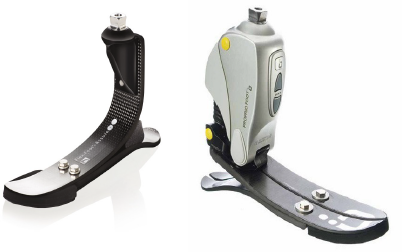
\includegraphics[height=2cm]{images/ccmp_01}

%\textit{Prothèse passive}
%\end{center}
%\end{minipage} \hfill
%\begin{minipage}[c]{.2\linewidth}
\begin{center}
\includegraphics[width=.5\linewidth]{ccmp_05}

%\textit{Prothèse active}
\end{center}
%\end{minipage} 



%\noindent\begin{minipage}[c]{.65\linewidth}
L'actionneur de la prothèse est un moteur à courant
continu alimenté par une batterie rechargeable de 16
Volts. L'énergie mécanique est transmise par un
réducteur de type poulies-courroie suivi d'un
système vis-écrou qui adapte cette énergie
mécanique pour la prothèse (ensemble de liaisons
entre le pied artificiel constitué d'une semelle en
fibres de carbone et le manchon ou tibia artificiel).
Des ressorts permettent d'ajuster également l'énergie
mécanique fournie au pied artificiel. L'effort exercé
par les ressorts est directement relié au couple
exercé par l'actionneur.

%La chaîne d'informations est constituée d'un
%ensemble de capteurs permettant d'acquérir
%différentes informations :
%\begin{itemize}
%\item un potentiomètre linéaire qui mesure
%l'allongement/écrasement du ressort;
%\item un codeur incrémental placé au niveau de
%l'articulation pied/tibia;
%\item plusieurs capteurs capacitifs disposés sous
%la semelle du pied au niveau du talon et
%à l'avant du pied.
%\end{itemize}
%\end{minipage} \hfill
%\begin{minipage}[c]{.3\linewidth}
%\begin{center}
%\includegraphics[width=\linewidth]{images/ccmp_05}
%\textit{Prothèse passive}
%\end{center}
%\end{minipage}


On peut modéliser la chaîne d'énergie de la façon suivante : 
\begin{center}
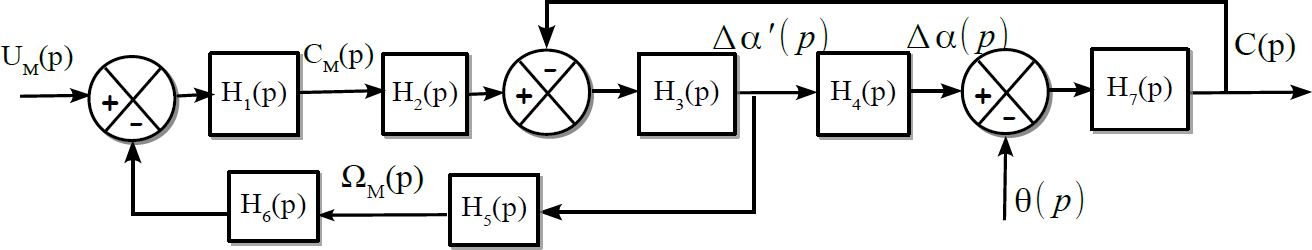
\includegraphics[width=\linewidth]{ccmp_07}
\end{center}

Les grandeurs temporelles sont les suivantes :
\begin{itemize}
\item $u_M$ tension d'alimentation du moteur (V);
\item $C_M$ couple exercé par le moteur (Nm);
\item $\omega_M$ vitesse angulaire du moteur (rad\, $\text{s}^{-1}$);
\item $\alpha$ angle de rotation du basculeur (rad) tel que $\alpha=\alpha_r+\Delta \alpha$ où $\alpha_r$ est la position repos et $\Delta \alpha$  est la variation angulaire autour de la position repos. On a alors : $\dfrac{\dd \alpha}{\dd t}=\dfrac{\dd \Delta \alpha}{\dd t}$. On note $\Delta \alpha' ( p)$ la transformée de Laplace de $\dfrac{\dd \Delta \alpha}{\dd t}$;
\item $\theta$ angle de rotation du pied (rad) tel que $\theta = \SI{0}{rad}$ pour la position repos;
\item $C$ couple exercé par le pied (Nm).
\end{itemize}
On note en majuscule, lorsque cela est possible, les variables associées aux grandeurs temporelles dans le
domaine symbolique.
%
%\subsection{Modélisation de la chaîne de transmission}
%\begin{obj}
%L'objectif de cette partie est de valider l'aptitude du système à reproduire un mouvement du pied à la
%vitesse angulaire maximale de \SI{5,2}{rad.s^{-1}} spécifiée dans le cahier des charges. Dans un premier temps, il
%s'agira de déterminer la relation entre la rotation du pied artificiel par rapport au tibia et la translation de la tige
%du vérin électrique. Dans un second temps, une analyse plus fine du fonctionnement du vérin électrique permettra
%de remonter à la vitesse angulaire du moteur.
%\end{obj}
%
%La vitesse angulaire maximale est atteinte durant la
%phase oscillante (le pied n'est plus en contact avec le
%sol). Durant cette phase, nous supposerons que le pied
%et le basculeur ne possèdent pas de mouvement relatif.
%Rechercher une relation entre $\theta$ et $\lambda$, revient donc à
%déterminer la relation entre $\alpha$ et $\lambda$.
%
%
%Le vérin électrique est mis en mouvement par l'intermédiaire d'un moteur électrique à courant continu. Le mouvement de rotation du moteur est adapté par l'intermédiaire d'un système poulies-courroie suivi d'un système vis-écrou. On note $\omega_M$ la vitesse angulaire du rotor du moteur par rapport au stator.
%
%\begin{center}
%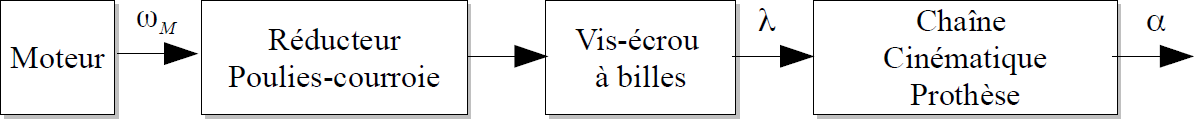
\includegraphics[width=\linewidth]{images/ccmp_08}
%\end{center}
%
%Le système vis-écrou est équipé d'une vis à billes de pas à droite $p_v$ avec $p_v=\SI{3}{mm.tour^{-1}}$. Le réducteur poulie-courroie possède un rapport de réduction $k=\dfrac{1}{2,1}$. On note $R_T$ le rapport entre la vitesse angulaire du rotor du moteur $\omega_M$ et la vitesse angulaire $\dfrac{\dd \alpha}{\dd t}$ tel que $\dfrac{\dd \alpha}{\dd t}=R_T\omega_M$.
%
%\question{En déduire les expressions littérales des blocs $H_4( p)$ et $H_5( p)$ . Déterminer la valeur numérique de $R_T$ . Conclure sur l'aptitude du moteur à générer la vitesse maximale exigée.}

\subsection*{Comportement dynamique de la prothèse}
\begin{obj}
L'objectif de cette partie est d'établir les équations de comportement dynamique de la prothèse autour de
la position de repos lors des phases d'appui et oscillante. Ces équations permettront de compléter le schéma-blocs
de la chaîne d'énergie.
\end{obj}

On donne l'équation différentielle linéarisée suivante qui caractérise le comportement dynamique de la prothèse :
$
J_M \dfrac{\dd^2 \Delta \alpha(t) }{\dd t^2} + \mu_m \dfrac{\dd \Delta \alpha(t) }{\dd t} = C_M(t)R_T -C(t)R_T^2$  avec  $R_T = \dfrac{1}{145}$.

Le moteur électrique est régi par les équations électriques et de couplage électromécanique :
\begin{itemize}
\item $u_M (t )=Ri (t)+e(t)$ avec $i (t )$ courant moteur et $e(t )$ fcem;
\item $e (t )=k_c \omega_M (t )$ avec $\omega_M (t )$ vitesse angulaire du rotor du moteur par rapport au stator;
\item $C_M (t )=k_c i (t )$.
\end{itemize}


%Les constantes intervenant dans ces équations sont définies dans le tableau suivant.
%
%
%\begin{center}
%\begin{tabular}{|p{.45\linewidth}|p{.45\linewidth}|}
%\hline
%Tension maximale $u_{\text{max}} =\SI{16}{V}$ & Résistance $R=\SI{1}{\Omega}$ \\ \hline
%Vitesse angulaire maximale sans charge $N_{\text{max}}=\SI{7600}{tr.min^{-1}}$ &
%Constance de couple $k_c=\SI{0,02}{NmA^{-1}}$ \\ \hline
%Couple maximal (pic) $C_{\text{max}}=\SI{2,5}{Nm}$ & Constante de fcem $k_e=k_c=\SI{0,02}{Vs}$ \\ \hline
%Courant sans charge : \SI{0,07}{A}  & Inertie du rotor $J_M=\SI{1,34e-5}{kg.m^2}$ \\ \hline
%\end{tabular}
%\end{center}

%\begin{center}
%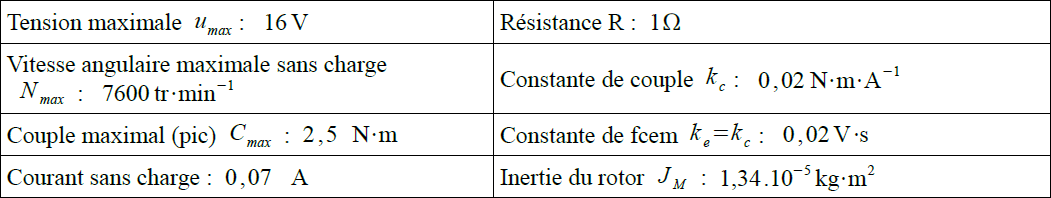
\includegraphics[width=.9\linewidth]{images/ccmp_06}
%\end{center}

\question{À partir des équations caractérisant le système, déterminer les expressions littérales des fonctions
de transfert $H_1( p)$, $H_2 ( p)$, $H_3 ( p)$ et $H_6 ( p)$.}
\ifprof
\begin{corrige}
On a d'une part, $C_M(p)=H_1(p)\left(U_M(p)-\Omega_M(p)\right)$. 

D'autre part, en utilisant les deux équations du moteur électrique, on a $U_M (p)=RI (p)+E(p)$ et $E (p )=k_c \Omega_M (p)$ soit  $U_M (p)=RI (p)+k_c \Omega_M (p)$. De plus $C_M (p)=k_c I (p )$; donc $U_M (p)=R\dfrac{C_M(p)}{k_c}+k_c \Omega_M (p)$. 
Par suite, $C_M(p)=\dfrac{k_c}{R}\left(U_M (p)-k_c \Omega_M (p)\right)$.

En identifiant, on a donc $H_1(p)=\dfrac{k_c}{R}$ et  $H_6(p)={k_c}$.


En utilisant l'équation différentielle caractéristique du comportement de la prothèse, on a : 
$J_M p^2 \Delta \alpha(p) + \mu_m p \Delta \alpha(p)  = C_M(p)R_T -C(p)R_T^2$
$\Leftrightarrow \Delta \alpha(p) \left(J_M p^2  + \mu_m p \right)  = C_M(p)R_T -C(p)R_T^2$.

D'après le schéma-blocs, 
$\Delta \alpha(p) = \left(C(p)-C_M(p)H_2(p)\right)H_3(p)H_4(p)$.

A TERMINER

\end{corrige}
\else
\fi

On a par ailleurs $H_4(p)=\dfrac{1}{p}$, $H_5(p)=\dfrac{1}{R_T}$ et $H_7(p)=k_{RS}d_0^2$ ($k_{RS}=\SI{1200e3}{N.m^{-1}}$ raideur équivalente du ressort et $d_0=\SI{0,035}{m}$).

On considère que $\theta(p)=0$. 

\question{Déterminer la fonction de transfert en boucle fermée $\text{FTBF}(p)=\dfrac{C(p)}{U_M(p)}$.}
\ifprof
\begin{corrige}
\end{corrige}
\else
\fi


%
%\subsection*{Identification d'un modèle de comportement de la chaîne d'énergie}
%
%\begin{obj}
%Le modèle de la chaîne d'énergie étant défini, on cherche maintenant à déterminer plus précisément les
%valeurs numériques des coefficients intervenant dans les fonctions de transfert de la chaîne d'énergie.\end{obj}
%
%\begin{minipage}[c]{.55\linewidth}
%On procède pour cela à une identification fréquentielle du
%comportement de la prothèse. L'expérience consiste à bloquer le
%tibia ainsi que le pied et à envoyer une commande en tension
%sinusoïdale au moteur en faisant varier la fréquence du signal.
%Dans ces conditions, le basculeur se déplace et écrase le ressort.
%On peut alors relever le couple $C$ au niveau de la cheville. On obtient alors les diagrammes de Bode
%donnés dans le document-réponse. Attention,
%l'abscisse est en hertz et le gain est normalisé
%$G_{\text{dB}}=20 \log\left( \dfrac{|H(p)|}{K_0}\right)$ . La courbe en tirets représente le modèle
%du second ordre déterminé précédemment s'approchant au mieux
%des courbes expérimentales.
%\end{minipage} \hfill
%\begin{minipage}[c]{.4\linewidth}
%\begin{center}
%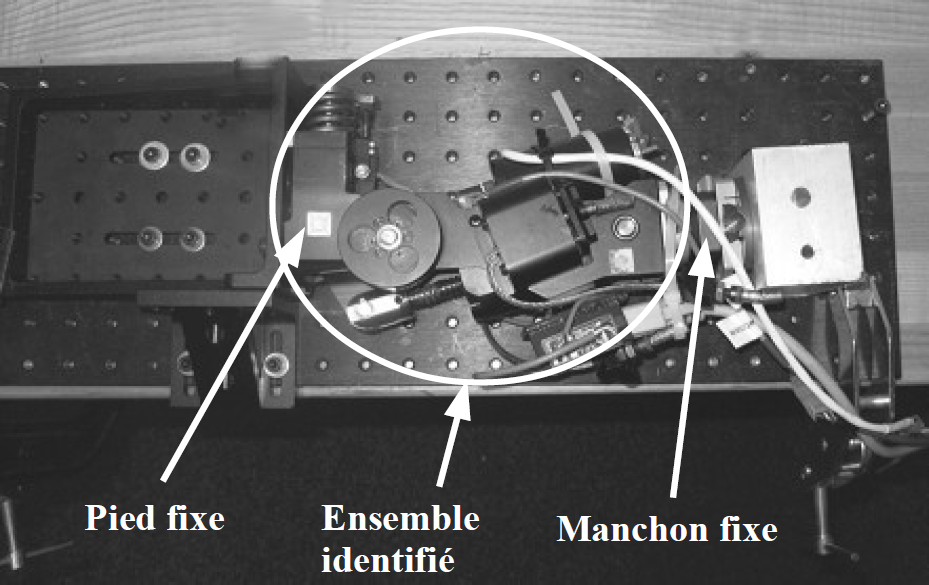
\includegraphics[width=\linewidth]{images/ccmp_03}
%
%\textit{Montage expérimental : pied et tibia (manchon) bloqués}
%\end{center}
%\end{minipage} 
%
%
%\subparagraph{}
%\textit{Déterminer les valeurs numériques de la pulsation propre non amortie $\omega_0$ et du coefficient
%d'amortissement $\xi_0$ à partir de la représentation approchée (courbe en tirets), en détaillant succinctement
%la méthode utilisée. Les tracés seront faits sur le document-réponse.}
%\ifprof
%\begin{corrige}
%\end{corrige}
%\else
%\fi
%
%\ifprof
%\else
%\newpage
%\if

\subsection*{Contrôler le processus lors de la phase d'appui}

\begin{obj}
La gestion des modes de commande permet de définir les séquences où l'asservissement s'effectue en
position et celles où l'asservissement s'effectue en couple. L'objectif de cette partie est de définir l'asservissement
en couple et d'analyser les performances de cet asservissement.
\end{obj}

\subsubsection*{Mise en place de l'asservissement en couple}
\ifprof
\else
On se place pour analyser les performances de l'asservissement en couple dans le cadre de l'expérience
d'identification décrite précédemment (pied et tibia bloqués).

L'asservissement en couple est réalisé grâce à un potentiomètre linéaire qui délivre une tension $u_{\text{mes}}$ image de la
variation de longueur des ressorts $\Delta X $. On note $K_{\text{capt}}$ le gain de ce capteur. D'autre part, un bloc d'adaptation de gain $K_A$ permet d'obtenir une tension $u_{\text{th}}$ image du couple de consigne $C_{\text{th}}$. L'écart $\varepsilon$ entre les tensions $u_{\text{th}}$ et
$u_{\text{mes}}$ est corrigé par un correcteur de fonction de transfert $H_c ( p)$ qui délivre la tension $u_M$ au moteur par
l'intermédiaire de l'amplificateur de gain $K_{\text{amp}}$.
\fi


\question{Compléter le schéma-blocs afin de mettre en place
l'asservissement en couple. Proposer une expression de $K_A$ permettant de réaliser un asservissement
correct.}
\ifprof
\begin{corrige}
\end{corrige}
\else
\fi

\begin{center}
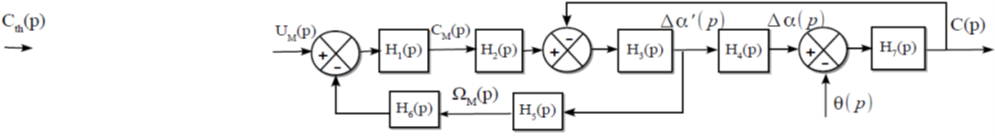
\includegraphics[width=\linewidth]{ccmp_09}

%\textit{Schéma-blocs de l'asservissement en couple simplifié}
\end{center}

\subsection*{Analyse des performances de l'asservissement en couple}

%\begin{minipage}[c]{.5\linewidth}
Le schéma-blocs de l'asservissement en couple peut être simplifié par le schéma-blocs suivant avec 
$H( p)=\dfrac{a_0}{1+a_1 p+a_2 p^2}$ où 
$a_0=\SI{2,9}{NmV^{-1}}$, 
$a_1=\dfrac{26}{4356}\SI{}{s}$ et $a_2=\dfrac{1}{4356}\SI{}{s^2}$ et $H_{\text{cor}}( p)=H_c (p)K_{\text{amp}}K_A$.
%\end{minipage} \hfill
%\begin{minipage}[c]{.4\linewidth}
\begin{center}
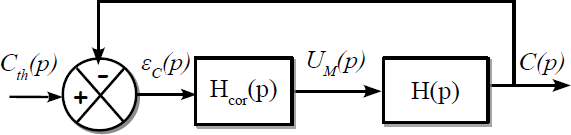
\includegraphics[width=\linewidth]{ccmp_04}

%\textit{Schéma-blocs de l'asservissement en couple simplifié}
\end{center}
%\end{minipage} 



\begin{obj}
L'objectif est de déterminer une correction  $H_{\text{cor}}( p)$ qui permette de respecter le cahier des charges
rappelé ci-après.
\end{obj}

\begin{center}
\begin{tabular}{|p{5.5cm}|l|}
\hline
Critères & Valeur \\ \hline\hline
Rapidité (temps de réponse à 5\%) & $t_{r5\%}<\SI{0,1}{s}$ \\ \hline
%Stabilité (marge de phase) & $M_{\varphi}=45\degres$  \\ \hline
Précision pour une entrée en échelon
(écart normalisé par la valeur de l'échelon) & 10 \% maxi \\
\hline
\end{tabular}
\end{center}

%
%
%On choisit dans un premier temps une correction proportionnelle telle que  $H_{\text{cor}}( p)= K_{\text{cor}}$.
%
%
%\subparagraph{}
%\textit{Déterminer l'expression de l'écart statique pour une entrée en échelon unitaire. En déduire la
%valeur de $K_{\text{cor}}$ notée $K_{\text{cor1}}$ qui permette d'assurer le critère du cahier des charges.}
%
%\vspace{.25cm}
%Les diagrammes de Bode de la fonction $H ( p)$ sont donnés dans le document-réponse.
%
%
%
%\subparagraph{}
%\textit{Déterminer graphiquement la valeur du correcteur proportionnel, notée $K_{\text{cor2}}$ pour assurer une
%marge de phase $M_{\varphi}=45\degres$ . Conclure sur l'aptitude du correcteur à vérifier les critères de précision et
%stabilité.}
%
%
%On retient finalement une correction telle que : $H_{\text{cor}}( p)= K_p+K_d \dfrac{\tau_d}{1+\tau_d p}$
%avec $K_p=\SI{4,3}{V.N^{-1}.m^{-1}}$, $K_d=\SI{20,6}{V.N^{-1}.m^{-1}}$ et $\tau_d=\SI{0,0016}{s}$.
%Les diagrammes de Bode de la Fonction de Transfert en Boucle Ouverte (FTBO) corrigée sont donnés sur le
%document-réponse. On réalise également une simulation pour une entrée en échelon de couple de
%\SI{50}{Nm} . La réponse indicielle du couple $C$ ainsi que l'évolution de la tension de commande de la prothèse $u_M$
%au cours du temps sont alors représentées.
%
%\subparagraph{}
%\textit{Tracer le diagramme asymptotique en le justifiant rigoureusement. }


{À l'aide des courbes, valider l'ensemble des critères du cahier des charges en justifiant clairement vos réponses. }

\begin{center}
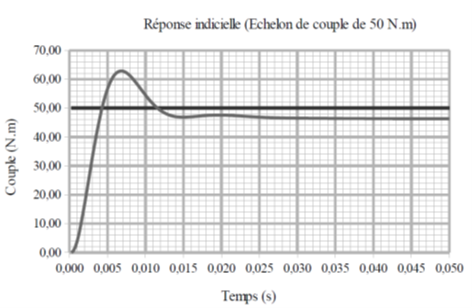
\includegraphics[width=\linewidth]{ccmp_10}

%\textit{Schéma-blocs de l'asservissement en couple simplifié}
\end{center}




\ifprof
\else
\begin{flushright}
\footnotesize{Corrigé  voir \ref{B2:07:77}.}
\end{flushright}%
\fi